% ****** Start of file apssamp.tex ******
%
%   This file is part of the APS files in the REVTeX 4.2 distribution.
%   Version 4.2a of REVTeX, December 2014
%
%   Copyright (c) 2014 The American Physical Society.
%
%   See the REVTeX 4 README file for restrictions and more information.
%
% TeX'ing this file requires that you have AMS-LaTeX 2.0 installed
% as well as the rest of the prerequisites for REVTeX 4.2
%
% See the REVTeX 4 README file
% It also requires running BibTeX. The commands are as follows:
%
%  1)  latex apssamp.tex
%  2)  bibtex apssamp
%  3)  latex apssamp.tex
%  4)  latex apssamp.tex
%
\documentclass[%
 reprint,
%superscriptaddress,
%groupedaddress,
%unsortedaddress,
%runinaddress,
%frontmatterverbose, 
%preprint,
%preprintnumbers,
%nofootinbib,
%nobibnotes,
%bibnotes,
 amsmath,amssymb,
 aps,
%pra,
%prb,
%rmp,
%prstab,
%prstper,
%floatfix,
]{revtex4-2}


\usepackage{gensymb}
\usepackage{graphicx}% Include figure files
\usepackage{dcolumn}% Align table columns on decimal point
\usepackage{bm}% bold math
%\usepackage{hyperref}% add hypertext capabilities
% \usepackage[mathlines]{lineno}% Enable numbering of text and display math
%\linenumbers\relax % Commence numbering lines

%\usepackage[showframe,%Uncomment any one of the following lines to test 
%%scale=0.7, marginratio={1:1, 2:3}, ignoreall,% default settings
%%text={7in,10in},centering,
%%margin=1.5in,
%%total={6.5in,8.75in}, top=1.2in, left=0.9in, includefoot,
%%height=10in,a5paper,hmargin={3cm,0.8in},
%]{geometry}



%%% USER ADDED PACKAGES

% user added packages 
\usepackage{xfrac}
\usepackage{mathtools}
\usepackage{subcaption}

\DeclarePairedDelimiter\bra{\langle}{\rvert}
\DeclarePairedDelimiter\ket{\lvert}{\rangle}
\DeclarePairedDelimiterX\braket[2]{\langle}{\rangle}{#1\,\delimsize\vert\,\mathopen{}#2}

%%% COMMANDS


\newcommand{\half}{$\sfrac{1}{2}$ }
\newcommand{\pauliz}{\begin{pmatrix}
                    1 & 0 \\
                    0 & -1 
                    \end{pmatrix}}
\newcommand{\halfpi}{\frac{\pi}{2}}


\begin{document}

\preprint{APS/123-QED}

\title{Nuclear Magnetic Resonance -- An Overview}

\author{Ali Ahmed}
\author{Zain Kamal}%
\author{Neil Mandar}%

\affiliation{%
    Department of Physics \& Astronomy, Rutgers University
}


\date{\today}% It is always \today, today,
             %  but any date may be explicitly specified

\begin{abstract}
bwaaa
\end{abstract}

\maketitle

%\tableofcontents

\section{\label{sec:intro}Introduction}

The study of nuclear magnetic resonance (NMR) utilizes weak magnetic fields to affect the nuclei of atoms in a strong magnetic field. Under certain conditions, atoms will exhibit ``resonance,'' causing the observation of a transient magnetic field as nuclei relax back to their equillibrium state. 

\section{\label{sec:theroy} Theoretical Description}

\subsection{\label{subsec:larmor} Larmor Precession}

We will start with the phenomena of Larmor precession, occuring when atoms are placed in a strong magnetic field. Larmor precession most readily occurs when the nucleus has a net magnetic moment i.e. there is an odd number of protons, producing a spin \half  system. In this case, the magnetic dipole moment $\mu$ of the nucleus is described as 

\begin{equation}
    \vec{\mu} = \gamma \vec{S}
\end{equation}

where $\vec{S}$ denotes the spin vector and $\gamma$ is a constant known as the gyromagnetic ratio (which differs depending on the type of nucleus). Under a magnetic field, the energy of this system reads 

\begin{equation}
    E = -\vec{\mu} \cdot \vec{B_0}
\end{equation}

where we denote $B_0$ the external magnetic field. This yields the Hamiltonian 

\begin{equation}\label{eqn:base-hamiltonian}
    H = -\gamma \vec{B_0} \cdot S
\end{equation}

where $S$ is the Pauli spin operator $S = (\sigma_x, \sigma_y, \sigma_z)$. Let us orient our magnetic field against the z-axis, such that 

\begin{equation}
    \vec{B_0} = B_0 \hat{z} 
\end{equation}

and the Hamiltonian now reads

\begin{equation}\label{eqn:hamiltonian}
    H = -\frac{\hbar}{2} \gamma B_0  \pauliz
\end{equation}

The Hamiltonian has eigenstates

\begin{equation}
    \ket{\pm} : E_\pm = \mp \frac{\hbar}{2} \gamma B_0 
\end{equation}

These eigenstates correspond to nuclei aligned either parallel or antiparallel to the magnetic field $B_0$. We will use these vectors $\ket{\pm}$ as our basis. We can evolve these stationary states with the time-dependent Schr\"odinger equation and then calculate the expectation of each of our Pauli matrices to obtain 

\begin{align*}
    \langle S_x \rangle &= \frac{\hbar}{2} \sin(\theta)\cos(\gamma B_0 t)\\
    \langle S_y \rangle &= \frac{\hbar}{2} \sin(\theta)\sin(\gamma B_0 t)\\
    \langle S_z \rangle &= \frac{\hbar}{2} \cos(\theta)   
\end{align*}

These equations are the classical precession equations; our spin vector will precess about the magnetic field at a constant frequency
\begin{equation}
    \omega_0 = \gamma B_0 
\end{equation}

This frequency is known as the \textbf{Larmor frequency}, and $\theta$ indicates the angle between $\vec{\mu}$ and $\vec{B_0}$. 

\begin{figure}[h]
    \centering
    {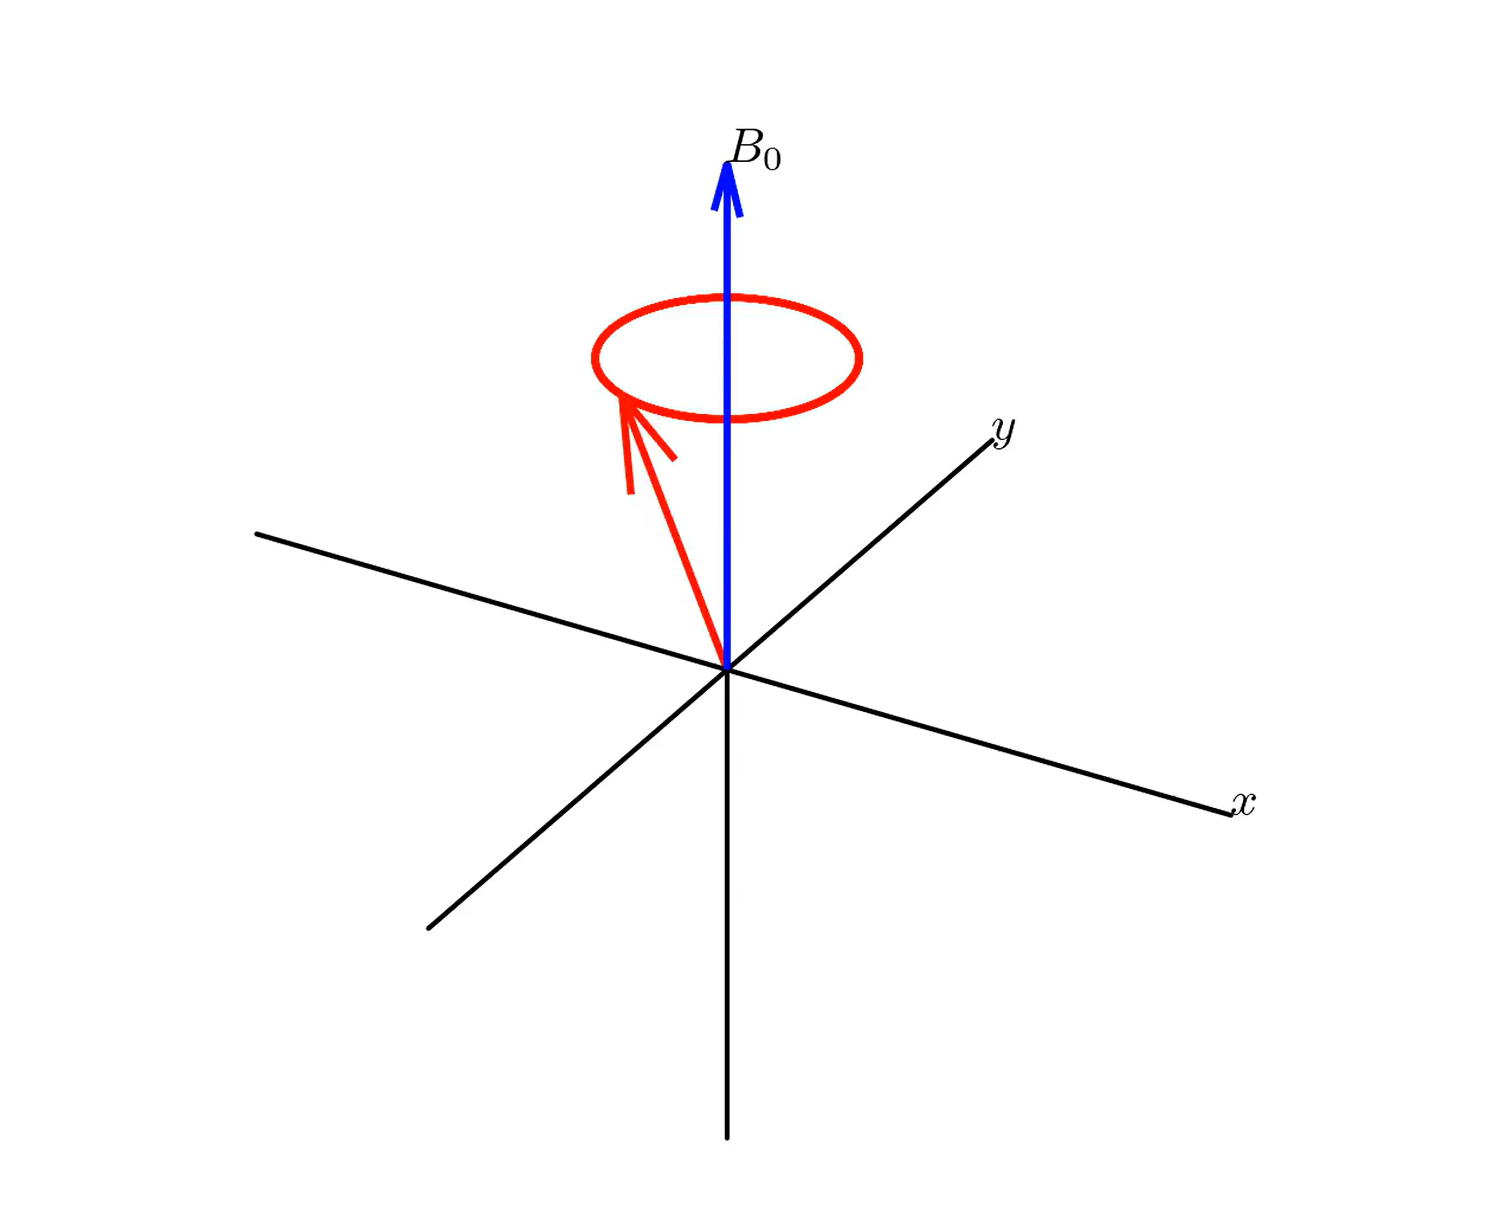
\includegraphics[width = 0.6\linewidth]{figs/larmor-precession.png}}

    \caption{Larmor precession about $\vec{B_0}$}
\end{figure}

$\theta$ characterizes the system, up to a phase,

\begin{equation}
    \ket{\psi} = \cos\left(\sfrac{\theta}{2}\right)\ket{+}+ e^{i\phi}\sin\left(\sfrac{\theta}{2}\right) \ket{-}
\end{equation}

These equations above can also be derived from a classical viewpoint; we can calculate the torque $\vec{\tau}  =\vec{ \mu }\times \vec{B_0}$ on the nucleus by the magnetic moment and use Newton's second law to derive a similar precession.

\subsection{\label{subsec:pulses} Net Magnetization and Relaxation}

The lower energy $E_+$ is the favored energy state; slightly more spins will align parallel to $\vec{B_0}$ as opposed to antiparallel. Using statistical mechanics, we can derive the expected number of $\ket{+}$ vs $\ket{-}$. Since this is a canonical two-state system, the ratio $\frac{N_+}{N_-}$ is equal to the ratio of the Boltzmann factors, yielding 

\begin{equation}
    \frac{N_+}{N_-} = \exp\left(\frac{\gamma \hbar B_0}{k T}\right)
\end{equation}

This small difference produces a net longitudinal magnetization (in this context, ``longitudinal'' refers ``along the $B_0$ field''), which is the sum of the individual quantized spins of the sytem. 

\begin{equation}
    M_z = \sum_i \gamma \hbar m_i = \frac{\hbar}{2} \gamma (N_+ - N_-)
\end{equation}

In equillibrium with our original magnetic field $B_0$, we expect a slight magnetization in the $+\hat{z}$ direction. However, if we were to apply another magnetic field briefly to this system, we would see a change in the net magnetization $\vec{M}(t)$. Eventually, the system will return back to its equillibrium state. In order to reach equillibrium, the system must give back energy to the surrounding lattice. 

We are interested in understanding how long it takes for our system to reach equillibrium. In general, after a disturbance, the magnetization follows the Bloch equation, reproduced in Equation \ref{eqn:bloch}

\begin{equation}\label{eqn:bloch}
    \frac{d \vec{M}(t)}{dt} = \frac{\vec{M}(t)-\vec{M_0}}{T_1}
\end{equation}

where $\vec{M_0}$ denotes the equillibrium magnetization. We refer to $T_1$ as the \textbf{spin-lattice relaxation time}.

\subsection{\label{sec:tipping}Producing Transverse Magnetizations}

\subsubsection{Apply a Circularly Polarized Field}

So far, we have discussed the uniform $\vec{B_0}$ field. However, to produce a transverse magnetization (i.e. a magnetization in the x-y plane) we need to get creative. We will use a circularly polarized field, 

\begin{equation}
    \vec{B_1}(t) = B_1\left[\cos(\omega_0t)\hat{x}+\sin(\omega_0t)\hat{y}\right]
\end{equation}

Note that $\vec{B_1}(t)$ oscillates at the Larmor frequency. Thus, the new Hamiltonian has an extra time-dependant term, still in the form of Equation \ref{eqn:base-hamiltonian}. Solving this Hamiltonian is beyond the scope of this lab report; however, can still apply the classical torque result 

\begin{equation}
    \vec{\tau} = \vec{\mu} \times \gamma \left[\vec{B_0}+\vec{B_1}(t)\right]
\end{equation}

by transforming into a rotating reference frame (rotating at the Larmor frequency), we find that the effective field becomes 

\begin{equation}
    \vec{\tau}^* = (B_0 - \sfrac{\mu}{\gamma}) \hat{z}^*+ B_1 \hat{x}^*
\end{equation}

In this rotating frame, applying a circularly polarized magnetic field has the effect of ``tipping'' the magnetization into a transverse plane. Transforming back into the lab frame, we will observe the magnetization in the x-y plane still precessing about the z-axis. 
\subsubsection{$\halfpi$ and $\pi$ pulses}

By applying $\vec{B_1}(t)$, we will create two types of pulses. We will first define a \textbf{$\halfpi$ pulse}, a pulse of $B_1(t)$ that will be applied for exactly long enough such that the magnetization is entirely in the $x-y$ plane. We will also define a \textbf{$\pi$ pulse}, a pulse that flips the magnetization from $+\hat{z}$ to $-\hat{z}$. 

During a $\halfpi$ or $\pi$ pulse, we can plot the expectation $\langle \vec{M} \rangle  = (\langle M_x \rangle, \langle M_y \rangle, \langle M_z \rangle)$ over time, as shown in Figure \ref{fig:pulse-spirals}.


\begin{figure*}[htbp]
    \centering
    \begin{subfigure}{0.3\linewidth}
        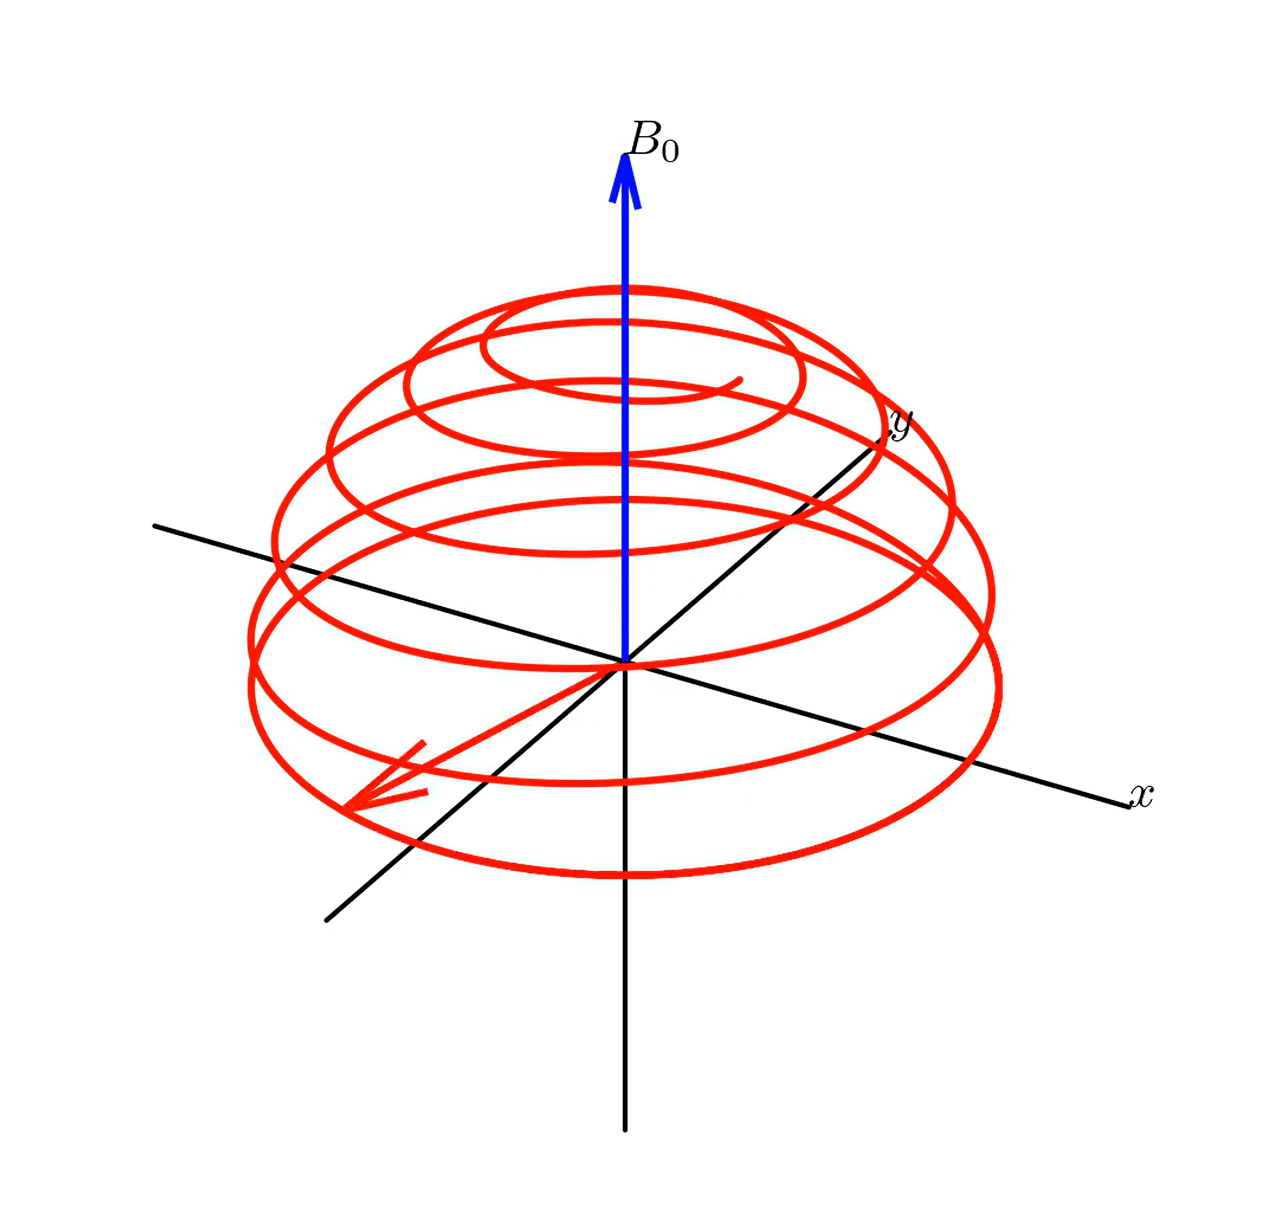
\includegraphics[width = \linewidth]{figs/pi-2-pulse.png}
        \caption{$\halfpi$ pulse produces transverse magentization}
    \end{subfigure}
    \begin{subfigure}{0.3\linewidth}
        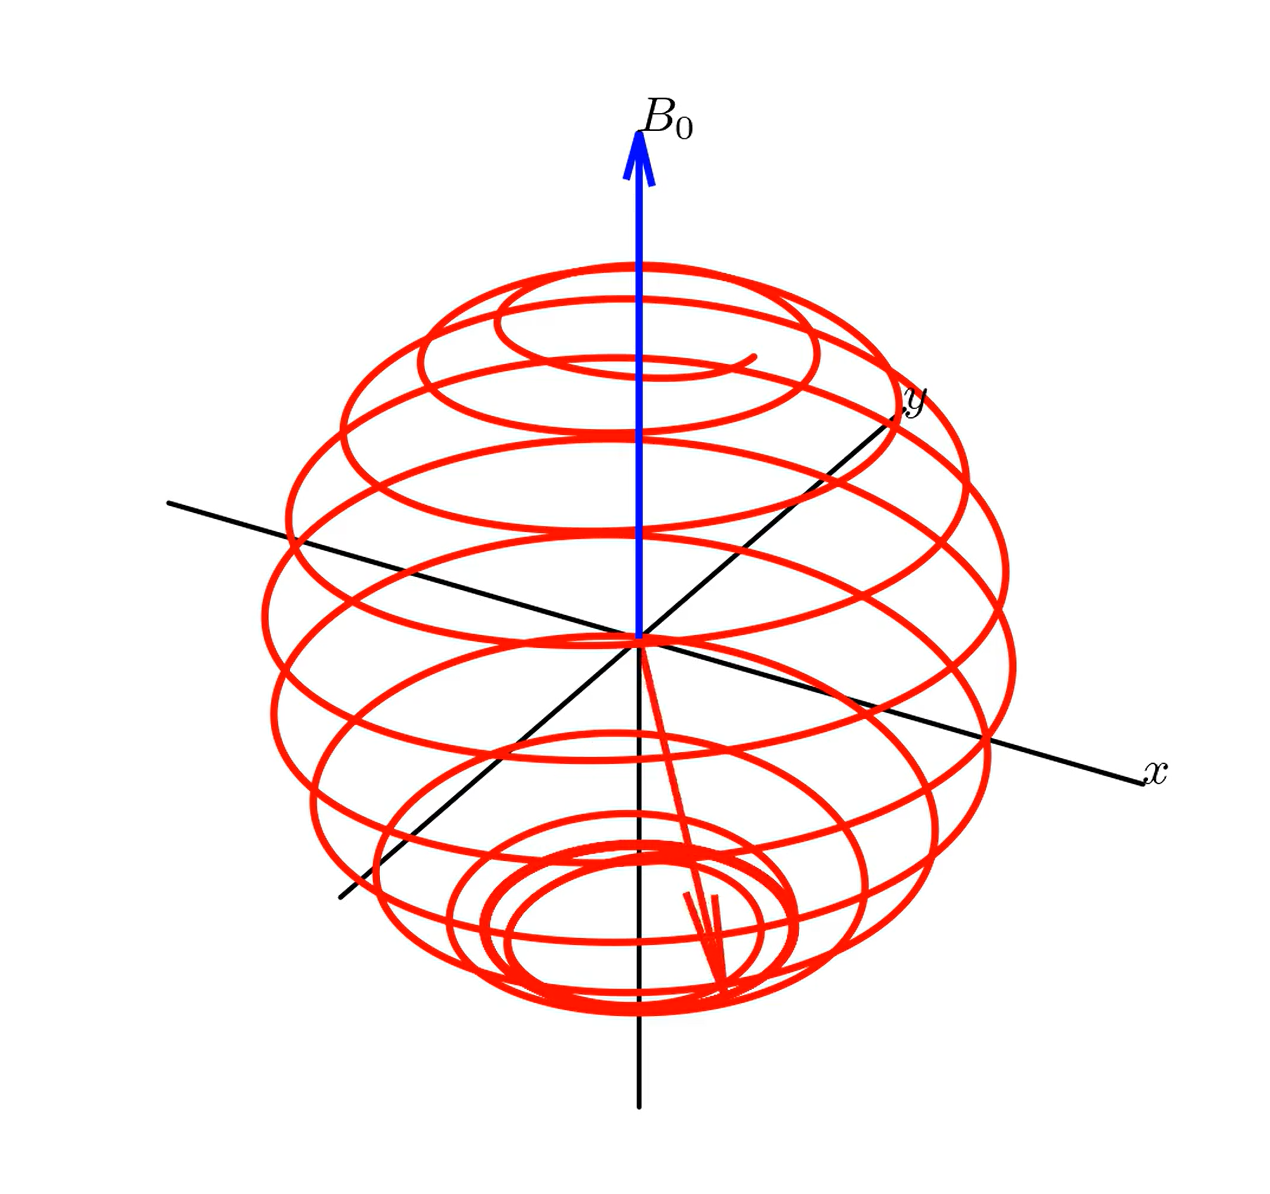
\includegraphics[width = \linewidth]{figs/pi-pulse.png}
        \caption{$\pi$ pulse flips magentization from $+\hat{z}$ to $-\hat{z}$}
    \end{subfigure}
    \caption{$\langle \vec{M} \rangle$ over time during a $\halfpi$ and $\pi$ pulse}\label{fig:pulse-spirals}
\end{figure*}

% The \nocite command causes all entries in a bibliography to be printed out
% whether or not they are actually referenced in the text. This is appropriate
% for the sample file to show the different styles of references, but authors
% most likely will not want to use it.
\nocite{*}

\bibliography{apssamp}% Produces the bibliography via BibTeX.

\end{document}
%
% ****** End of file apssamp.tex ******
